% Chapter 1

\chapter{Quantum computing in silicon: A different way of computation} % Main chapter title

\label{Chapter1} % For referencing the chapter elsewhere, use \ref{Chapter1} 

\HRule
\vspace{0.5cm} \hspace{2cm}
\small
\hangindent=4cm
\\
        ``\emph{Second quantum revolution. The definition of insanity is doing the same thing over and over and expecting different results.}" 
\\ \\
\hangindent=4cm
\begin{flushright}
--Unknown \\
\end{flushright}

\vspace{0.5cm}

\noindent \HRule
\clearpage



%----------------------------------------------------------------------------------------

% Define some commands to keep the formatting separated from the content 
\newcommand{\keyword}[1]{\textbf{#1}}
\newcommand{\tabhead}[1]{\textbf{#1}}
\newcommand{\code}[1]{\texttt{#1}}
\newcommand{\file}[1]{\texttt{\bfseries#1}}
\newcommand{\option}[1]{\texttt{\itshape#1}}

%----------------------------------------------------------------------------------------


\section{Introduction: The quantum revolution of computation}

Ever since the invention of the abacus around 2700-2300BC in Babylon \cite{abacus} computation has been a fundamental pillar of human society. Over centuries calculus and mathematics has evolved and become more and more relevant in all kinds of aspects of our lives. When in the second half of the 20th century the digital computer was invented, data processing and stored capabilities grew exponentially, following Moores Law which predicts an increase of processing power by a factor of two per year. \cite{MooresLaw} This in turn revolutionized many aspects of modern life, like logistics, medicine, weather forecasting, banking and many more. But also is computing constantly reinventing itself, e.g. with the invention of the internet in 1990. \cite{The conversation https://theconversation.com/the-history-of-computing-is-both-evolution-and-revolution-57126 } Nowadays computing is deeply embedded in every day life where humans created big data. This is fed to computers and then in turn impacts people. Thus we rely on this ever improving technology, but this is the point where we run into trouble. Not only is Moores Law is approaching a critical point after which is might break down, the quantum limit, but also are some key problems of modern society, like data-searching, simulating large chemical (or quantum) systems or predicting material properties, computationally hard - meaning that they will never be solved by a classical computer, regardless of its power. 
This is the frontier of complexity as John Preskill calls it. \cite{JohnPreskillNasa}
So if quantum mechanics becomes relevant for computer chips of incredibly small size and quantum systems are hard to simulate, why shouldn't we fight fire with fire and use quantum properties for computing to tackles these problems and reach the next stage of computing?
Already in 1982 physicist Richard Feynman suggested this approach "Nature isn't classical, […], and if you want to make a simulation of nature, you'd better make it quantum mechanical, and […] it's a wonderful problem, because it doesn't look so easy." This idea has far reaching implications for the hardware necessary to realise this quantum computation - it also needs to exhibit quantum mechanical properties. Thus the classical bits are replaced by quantum bits (qubits). Unlike classical bits,  qubits have two inherent quantum mechanical properties that give quantum information its power: superposition and entanglement. The former means that the qubit can be in exclusive states, like the binary 0 and 1, at the same time. The latter describes the correlation between different states - fully entangled states cannot be described independently, they are not separable. 
Combining this two aspects of quantum mechanics makes quantum information powerful as now highly parallel processing is possible as N qubits have $2^N$ eigenstates which can be used simultaneously.   
The foundation of this is the qubit. This needs to be a well-defined two-level system, that can interact strongly with another qubit but does not interact strongly with the environment, except for measurements. This already gives us an indication that this is indeed a challenging task like Feynman already suggested, but the implications are so large that in the last decades not only researchers but also companies like IBM, Intel, Microsoft and Google have started to participate in the race for a quantum computer. Billions of dollars are invested every year for the potential to simulate quantum systems and thus develop new drugs, more efficient fertilizers and much more. Everyone wants to achieve the quantum revolution of computation and in the following chapters I will describe how this work brings us one step closer towards this aim. 

%a bit more about algorithms, simulation, qp hard and such?

%----------------------------------------------------------------------------------------

\section{Foundation: the qubit}
 

\subsection{An introduction to the qubit}

\cite{Smith2017}
A qubit consists out of a well-defined quantum two levels system. This is defined by its Hamiltonian $\mathcal{H}$, an operator which corresponds to the total energy of the system. The two levels are described by the eigenstates of this system $\ket{0}$ and $\ket{1}$. The qubit can then by in any superposition state $\ket{\psi}=\alpha\ket{0}+\beta\ket{1}$ with $\alpha\in\mathds{C}$ and $|\alpha^2|+|\beta^2|=1$. While this superposition state can be used during operations, it can never be observed. Whenever a quantum particle's state is measured, the part of the wave function associated with that state then collapses into a single eigenstate with a single eigenvalue, in this case either $\ket{0}$ or $\ket{1}$. The probability to collapse into this states is respectively $|\alpha|^2$ and $|\beta|^2$. Thus, to readout a quantum state, a temporal ensemble measurement is performed by repeating the whole process many times. \footnote{For completeness, a spatial ensemble measurement is also possible.} 

A qubit can be represented geometrically as a vector in three-dimensional space, where the mutually orthogonal eigenstates $\ket{0},\ket{1}$ are typically positioned on the north and south pole respectively. All points on the surface of the sphere symbolize pure superpositions of the eigenstates while interior points signify mixed states. This construct is called Bloch sphere and shown in figure \ref{fig1:Blochsphere}. 

There exist plenty two-level system in different physical systems. However, to viably implement a qubit a number of criteria need to be fulfilled at a minimum. DiVincenzo first devised  these guidelines. \cite{DiVincenzocriteria} 
The qubit itself must be well-defined, aka describable by an Hamiltonian, as well as have a well-defined known initial state in which it can be prepared with high precision before starting an operation. Furthermore, one needs to be able to measure the qubit, thus being able to read-out the value of the qubit precisely at any time. Moreover, a universal set of quantum gates has to exist for one and two qubits to execute quantum algorithms. On contrast the qubit needs to be isolated from its environment to prevent fluctuations on the outside to change the quantum state, leading to a loss of state coherence. This coherence needs to be much smaller than the gate operation time.  Lastly the qubits have to form a scalable architecture where many qubits can interact with each other, long distance transport of qubit states is possible and errors can be corrected.
Notice that while qubits are the most common way to attempt building a quantum computer, quantum d-state systems or continuous quantum variables also seem to be a viable option \cite{Ladd2010}. 
 
There exist a myriad of physical systems that promise to fulfil these criteria  reaching from microscopic systems such as trapped atoms, photons and spins in semiconductors to macroscopic systems such as superconducting qubits. \cite{Ladd2010}
As it stands, trapped ions and superconducting qubits are leading the race in form of number of connected qubits, reaching 50 and 49 respectively\cite{50qubits, 49qubits}. However, if these platforms will establish themselves in the long run is still in question as trapped ions are challenging to scale up to large qubit networks and superconducting qubits struggle with ???\cite{idk}. One very promising and growing sector are semiconductor spin qubits, specifically silicon based ones. Due to the facts, that firstly, they are compatible with the current billion dollar semiconductor industry and secondly, they have potential for large scale quantum computing as they are small but still flexible. DiVincenzo and Daniel Loss first proposed a single spin qubit in 1999\cite{Loss1998}. Shortly after, the first GaAs spin qubit was build in 2004\cite{Elzerman2004} and has seen huge development since \cite{Koppens2006, Petta2005, ...}. However, silicon  has always been the dream qubit material as its industry nano-processing capacities are far superior and it lacks the intrinsic nuclear magnetic field which makes GaAs difficult to work with. In 1998 Kane already proposed a silicon based quantum computer \cite{Kane1998}, but it took until 2007 for the first single electron occupation quantum dot  \cite{Simmons2007} to be realised. Since then phosphorus donor based qubits \cite{Morello2010}, CMOS qubits \cite{Feldhorst} and SiGe qubits \cite{Tarucha} have been devised reaching high levels of accuracy and control \cite{??}. 
The focus of this thesis is the single spin donor based qubit in silicon.

\subsection{Phosphorus dopants in silicon} \label{sec:silicon}

Crystalline silicon is bonded convalently with a diamond structure. Its band structure is drawn in figure \ref{fig:bandstructure} and shows that the conduction band minimum is at a momentum of $k_0=0.85k_0$ with $k_0=1/a_0$ as the Brillouin zone boundary and such has an indirect band gap. This minimum has a six-fold degeneracy due to the cubic symmetry of bulk silicon. We call this 6 conduction band minima valleys. In nanodevices the degeneracy can be lifted due to breaking of symmetry. Specifically, for an electron bound to a donor positioned in the silicon lattice, the strong confinement potential created by the dopant atom, lifts breaks the cubic symmetry and lifts the degeneracy so that the six levels split into a singlet ground state A1 and a triply (T2)- and doubly-degenerate (E) set of excited states as portrayed in figure \ref{fig:sivalleys} (b). 

\begin{figure}
\centering
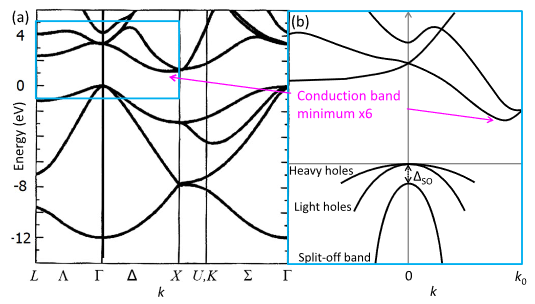
\includegraphics[width=\columnwidth]{bandstructure}
\caption{
bandstructure
}
\label{fig:bandstructure}
\end{figure}
 


\begin{figure}
\centering
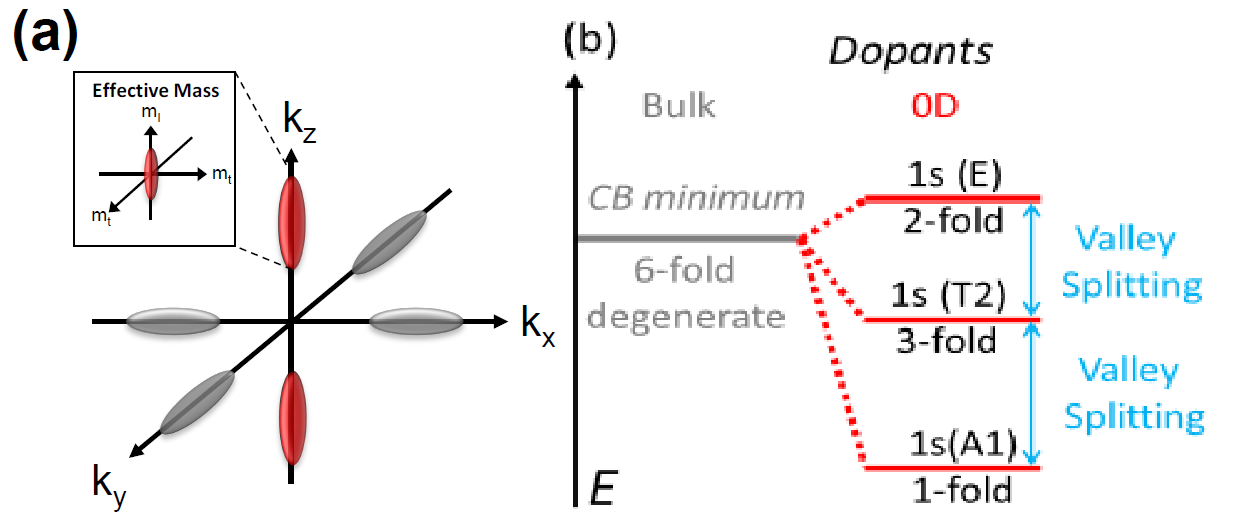
\includegraphics[width=\columnwidth]{SiValleys}
\caption{
Valleys in silicon. (a) Conduction band band minima in bulk silicon, showing six ellipsoids
(valleys) in the Brillouin zone. Inset : The components of the effective masses (for the valley kz ), along three
directions in k-space, highlighting the longitudinal (ml ) and transverse (mt ) masses. (b) The degeneracy
of the 6 valleys broken by confinement, strain and sharp interfaces, highlighting the orbital ground states
separated by valley splitting. 
}
\label{fig:sivalleys}
\end{figure}
 

\subsection{The Phosphorus donor spin qubit} \label{sec:donorqubit}

Spin is an intrinsic quantum mechanical property of elementary particles and atomic nuclei that describes how the particle is deflected when moving in magnetic fields. It gives the particle angular momentum and a small magnetic moment. Spin is quantized, thus can only take discrete values $-s, -s+1, ..., s-1, s$ where $s=\frac{n}{2}$ is the spin quantum number with $n\in \mathds{N}_0$. This makes spin $s=1/2$ ideal for quantum computation, being a natural two level system. 
A particle with spin $1/2$ is the electron. The excess electron of a donor in silicon can be used for this purpose. In this environment the donor atom in the semiconductor can be treated analogous to a hydrogen atom in vacuum with a few modifications \cite{Zwanenburg}.
E.g. due to the broken symmetry the dispersion relation for electrons near the bottom of each valley is anisotropic and is described by two light traverse effective masses (mt = 0.19m0) and a heavy longitudinal effective mass (ml = 0.98m0), where mo is the mass of the free electron \cite{d}. This is illustrated in figure \ref{fig:sivalleys} (a).  


\begin{figure}
\centering
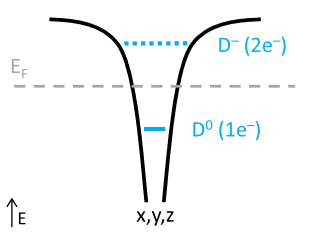
\includegraphics[width=0.5\columnwidth]{confinement}
\caption{
Donor confinement potential. 
}
\label{fig:donorconfinement}
\end{figure}


Phosphorus is a convenient donor for silicon as its nucleus also carries spin $1/2$ which gives us a second qubit "for free". 
The spin states $\pm \frac{1}{2}$ of the electron and the nucleus will be called $\{\ket{\uparrow}$, $\ket{\downarrow}\}$ and $\{\ket{\Uparrow}$, $\ket{\Downarrow}\}$ respectively. Unperturbed these spin states have the same energy - they are degenerate. However, if an external magnetic field $B_0$ is applied they split by the Zeeman energy $E_z=\gamma B_0$, with $\gamma$ being the corresponding gyromagnetic ratio, making them accessible as qubits. The Hamiltonian describing this system is 
\begin{equation}
H_Z=\gamma_e B^z_0 \mb{S}_z-\gamma_N B_0^z \mb{I}_z
\end{equation}
with $B_0^z$ as the component of the magnetic field along the z-axis, $\{\mb{S}_z,\mb{I]}_z\}$ the spin operator in z direction of the electron and nucleus respectively and $\gamma_e=28\,$GHz/T, $\gamma_N=17\,$MHz/T as the respective gyromagnetic ratios.

However, the electron and the nucleus are not separated from each other but interact intrinsic due to the hyperfine interaction $A$. This interaction arises from the wave function overlap of the singlet electron ground state A1 and the nucleus and adds an interaction term $A\mb{S\cdot I}$ to the Hamiltonian

\begin{equation}
H=H_z+H_A=\gamma_e B^z_0 \mb{S}_z-\gamma_N B_0^z \mb{I}_z + A\mb{S\cdot I}
\end{equation}
The excited electron valley states have zero probability at the nucleus and thus do not exhibit hyperfine interaction. 
For the conditions $\gamma_eB_0^z \ll A>\gamma_N B_0^z $ which imply that the detuning between the coupled states $\ket{\uparrow\Downarrow},\ket{\downarrow\Uparrow}$ is much larger than the hyperfine coupling, the electron and nuclear states can be separated and the eigenstates of the Hamiltonian $\ket{\uparrow\Uparrow},\ket{\uparrow\Downarrow},\ket{\downarrow\Uparrow},\ket{\downarrow\Downarrow}$ are the tensor products of the individual spin states $\ket{\uparrow\Uparrow}=\ket{\uparrow}\otimes\ket{\Uparrow}$ etc. 
In figure \ref{fig:energydiagram} the energy levels of the eigenstates are displayed. 

\begin{figure}
d
\end{figure}


\subsection{Electron qubit initialization and measurement}\label{sec:qubit_initMeas}
\footnote{The nuclear qubit can be mapped onto the electron with pulses discussed in the paragraph "Qubit control" and thus relies on the same principles.}
To successfully operate the spin system as qubits, one needs to be able to determine in which spin state it is at any given time. To achieve this, we convert the electron spin signal into a charge signal, known as spin to charge conversion and then electrically read out the charge signal with off the shelve electronics.

To convert from spin to charge the spin states of the electron are tuned with bias voltages such that the Fermi level of a neighbouring reservoir lies in between both states like shown in figure \ref{fig:spintocharge}. In this case $\ket{\uparrow}$ will tunnel into the reservoir and be replenished by $\ket{\downarrow}$ while $\ket{\downarrow}$ will stay at the donor. As this tunnel process is a moving charge, we have now converted the spin signal into a charge signal. 

The key feature to now readout this charge signal is the single electron transistor (SET). This is a nanometric structure which can form an island of hundreds of electrons. The island is capacitively coupled to a top gate and tunnel coupled to source and drain reservoirs as shown in figure \ref{fig:SET}. The energy of this island is 
\begin{align*}
E & =  \frac{Q^2}{2C}\\
& =  \frac{e^2N^2}{2C}\\
& =  E_C N^2
\end{align*}
where Q is the charge of island which consists out of N electrons, C is the total capacitance of the dot and $E_C$ the charging energy. 
To add one electron one needs the energy 
\begin{align*}
\Delta E(N)& =  E(N+1)-E(N)\\
 & =  E_C\left(N+\frac{1}{2}\right)
\end{align*}
also called the electrochemical potential $\mu(N)$. Transport, thus current flow, occurs when the electrochemical potential to add the Nth electron lies between the Fermi levels of the source and drain reservoirs as shown in figure \ref{fig:SET2}. If transport is blocked, the SET is in Coulomb blockade. By varying the top gate voltage oscillations between high and low current occurs when single electrons tunnel, which are called Coulomb oscillations and are shown in figure \ref{fig:coulomboscillations}. Due to the sharp slope of these curves, the sensitivity of the SET current to changes in the electrostatic environment is very high. Thus a change in charge on the donor due to a spin tunnelling event will result in a change in current on the SET. Consequently we can readout the electron qubits  spin state. This is shown in figure \ref{fig:blips}. 

This measurement process can also be used to initialize the qubit into a well known state, a vital feature for qubit operation, as at the end of the process always $\ket{\downarrow}$ is occupying the donor. 

This has been first demonstrated on a single electron spin on a phosphorus donor in 2010 by A. Morello who showed single shot readout.\cite{Morello2010}

\paragraph*{Qubit control} \label{sec:qubit_control}
To control the qubits we use magnetic resonance. As mentioned above, spins have a magnetic momentum and react to external magnetic fields. More precisely they precess around the axis of magnetization with a frequency $f_L$, the so called Larmor frequency. Now we apply a magnetic pulse oscillating with a frequency $f_{ac}$. In the reference frame of this oscillating  field, also known as the rotating frame, the spin appears to precess at a frequency $\Delta f=f_L-f_{ac}$.  If a magnetic drive with the same frequency as the Larmor frequency is applied perpendicular to $B_0^z$, it appears in the rotating frame as a static field of amplitude $B_1$ in the x-y plane. If the spin has been prepared in either $\ket{\uparrow}$ or $\ket{\downarrow}$, the spin will rotate around the axis of $B_1$ with frequency $f_{Rabi}=\gamma B_1$, the Rabi frequency, as these rotations are called Rabi oscillations. This is shown in figure \ref{fig:rabi}. 
When this magnetic resonance technique is applied to the electron, we speak of electron spin resonance (ESR) and when it is applied to the nucleus of nuclear magnetic resonance (NMR).
In figure \ref{fig:leveldiagram} these magnetic transitions and their resonance frequencies are illustrated. 
For the phosphorus donor electron qubit this was first demonstrated in 2012\cite{Pla2012} and for the nuclear qubit in 2013.\ref{Pla2013}

%extend more in preparation for flipflop?


\paragraph*{Qubit decoherence} \label{sec:decoherence}

Quantum decoherence is the loss of quantum information from a system, in our case the qubit, to the environment.
This happens as the qubit is never fully isolated from its environment and interactions lead to the transfer of information from the qubit to the outside. 

There are two main parameters which describe the lifetime of the qubits quantum information. 

Firstly, there is the relaxation time $T_1$ which is the time scale on which the qubit decays from its excited state $\ket{\uparrow}$ to its ground state $\ket{\downarrow}$ due a perturbation orthogonal to the quantization axis, in the case of the donor qubit this means a perturbation of type $\sigma_{x,y}$. This perturbations can e.g. arise due to charge fluctuations and tunnelling effects. More about the specific effect of this process on our qubit, its origins and how to mitigate it will be discussed in chapter \ref{chap:t1}. 

Secondly, there is the randomization of the phase of a quantum superposition on the time scale $T_2$, which is called dephasing. Slow perturbations along the quantization axis $\sigma_z$ cause the Larmor frequency to fluctuate and the state starts precessing in the rotation frame such that we loose track of the phase of the state. 
In ensemble measurements a third time scale is relevant, the dephasing time $T_2^*$, where different parts of the ensemble have different Larmor frequencies due to slow fluctuations. As we are working with single spins, we only encounter time ensemble measurements. In these cases the Larmor frequency varies between each measurement due to slow changes in the environment in between. This dephasing can be suppressed by clever pulsing methods like hahn echo and CPMG \cite{CPMG}. 

Both the electron and the nuclear spin have exceptionally long coherence times when placed in an environment with few surrounding spins, as was first measured by J. Muhonen in 2014 \cite{Muhonen2014}. In combination with the high fidelity control, this makes for an excellent qubit.  

%more reference?

%----------------------------------------------------------------------------------------

\section{Approach to large scale quantum computing} \label{sec:scaleup}

\subsection{Surface Code}

\section{Circuit Quantum Electrodynamics}

\section{Scope of this thesis}


